% This is a LaTeX thesis template for Monash University.
% to be used with Rmarkdown
% This template was produced by Rob Hyndman
% Version: 6 September 2016

\documentclass{monashthesis}

%%%%%%%%%%%%%%%%%%%%%%%%%%%%%%%%%%%%%%%%%%%%%%%%%%%%%%%%%%%%%%%
% Add any LaTeX packages and other preamble here if required
%%%%%%%%%%%%%%%%%%%%%%%%%%%%%%%%%%%%%%%%%%%%%%%%%%%%%%%%%%%%%%%

\author{Beinan Xu}
\title{What makes a good prediction interval or probabilistic forecast?}
\studentid{26401746}
\def\degreetitle{Masters of Applied Econometrics}
% Add subject and keywords below
\hypersetup{
     %pdfsubject={The Subject},
     %pdfkeywords={Some Keywords},
     pdfauthor={Beinan Xu},
     pdftitle={What makes a good prediction interval or probabilistic forecast?},
     pdfproducer={Bookdown with LaTeX}
}


\bibliography{thesisrefs}

\usepackage{amsthm}
\newtheorem{theorem}{Theorem}[chapter]
\newtheorem{lemma}{Lemma}[chapter]
\theoremstyle{definition}
\newtheorem{definition}{Definition}[chapter]
\newtheorem{corollary}{Corollary}[chapter]
\newtheorem{proposition}{Proposition}[chapter]
\theoremstyle{definition}
\newtheorem{example}{Example}[chapter]
\theoremstyle{definition}
\newtheorem{exercise}{Exercise}[chapter]
\theoremstyle{remark}
\newtheorem*{remark}{Remark}
\newtheorem*{solution}{Solution}
\begin{document}

\pagenumbering{roman}

\titlepage

{\setstretch{1.2}\sf\tighttoc\doublespacing}

\clearpage\pagenumbering{arabic}\setcounter{page}{0}

\chapter*{Abstract}\label{abstract}
\addcontentsline{toc}{chapter}{Abstract}

This thesis is about introducing scoring rules and using it to evaluate
interval forecasts and probabilistic forecasts. In the past few decades,
the interval forecasts and probabilistic forecasts have a very important
development and are attracting more and more attention. More and more
organizations and individuals begin to use probability prediction
instead of point prediction to carry out the future. However, the
traditional evaluation methods of point prediction cannot effectively
evaluate the results of probabilistic prediction. Because if we want to
evaluate the probability prediction effectively, we should not only
evaluate the sharpness of the prediction distribution but also evaluate
its calibration. For evaluating the result of interval forecasts and
probabilistic forecasts, scoring rules is a very effective method. It
can evaluate the sharpness of the prediction of distribution while
assessing calibration. In this article, we have used different scoring
rules to evaluate the different forecasting result base on different
models at the index of ASX 200 and M3 datasets.

\chapter{Introduction}\label{ch:intro}

In this world, people wish to understand the future development from
different events. For example, residents want to know tomorrow's weather
and temperatures to decide what kind of clothes they need to choose.
Securities investors want to know the future price trend of securities
in order to formulate a suitable investment portfolio. Unfortunately, it
is very difficult for humans to predict the future because uncertainty
is a universal feature of this world. Although we have a variety of ways
to predict future events, such as building suitable time series models
based on past information, then predicting future trends over time, none
of these methods provide absolutely accurate future predictions. The
limitations are that, first of all, various activities and phenomena in
the real world are difficult to be perfectly represented by mathematical
models, especially humanistic phenomena such as the purchase of lottery
tickets (the outcome of the lottery is random). Although there are some
natural phenomena, they have certain rules to follow, such as
temperature have seasonal changes, so it is very difficult to establish
prediction models for them. Second, human cognition is limited. For the
an event, people cannot collect and obtain all of information for the
relevant factors. Because of these limitations, using these methods to
make predictions must not be absolutely accurate. For now, to accurate
forecast future is still a difficult task, but as more and more
prediction methods and models are developed, forecasters can use them to
get what they want. The following problem is how to evaluate these
models, because choosing the correct assessment method can effectively
compare the accuracy of forecast results by using different models, then
the forecaster can obtain the most suitable prediction model.

In choosing the forecast method, point forecast is the most commonly
used. But forecasts should be probabilistic (\textcite{GK14}) and point
estimation gradually transform to distribution estimation
(\textcite{S75}). Therefore, interval forecasts and probabilistic are
being used more and more frequently. Probabilistic prediction is a
method to forecast future uncertain events and development by generating
probability prediction distribution. Base on the available information
set, to maximize the sharpness of prediction distribution and subject to
calibrate. (\textcite{GK14}) Comparing the point forecasts can produce a
single point result, such as predicted a stock price in the next day,
probabilistic prediction can supply more information to the forecaster
by assigning a probability distribution to each future possible outcome
as supplying the probabilistic distribution on different prices on the
second day. Obviously, probabilistic forecasting has more obvious
advantages than point forecasting, so people begin to use probabilistic
forecasts to predict activities rather than using point forecasts in
many fields, such as finance, weather, medicine etc. In the
\textcite{R16} paper, it discussed five potential predictors who have a
need for probability forecasts.

For evaluating the accuracy of point forecast results, the common ways
are to calculate the forecast errors, scale-dependent errors (as Mean
absolute error, Root mean squared error), percentage errors (as Mean
absolute percentage error) or scale errors (as mean absolute scaled
error) (\textcite{RA18}). But for interval forecasts and probabilistic
forecasts, the scoring rules are used more generally. At present,
scoring rules are mainly used in weather forecasting system. They
provide such an assessment by giving a numerical score based on
probability and actual observation (\textcite{W96}) and proper scoring
rules encourage the forecaster to conduct careful assessment and honesty
(\textcite{GR07}).

This thesis introduces the scoring rules in Chapter 2. In this Chapter,
probability forecasts, sharpness and calibration is reviewed. Also
interval scoring rules and distribution scoring rules are reviewed
separately, and they are applied to evaluate interval forecasts and
probability forecasts respectively. Meanwhile, the corresponding formula
and derived formula are shown in Chapter 2.1 and 2.2. In the third
chapter, after using two different models to fit the financial data,
interval forecast and probabilistic forecast are performed separately.
Then the prediction results are evaluated by using suitable interval
scoring rules and distribute scoring rules.In the same way, in Chapter
4, we select M3 data sets that have more abundant data types, and choose
more different models to make forecasts, then to evaluate.

\chapter{Assessing probabilistic forecasts using scoring
rules}\label{assessing-probabilistic-forecasts-using-scoring-rules}

The traditional prediction method is mainly based on point forecasts,
which can provide forecasters with future development trend information
under given significant level. But the future is extremely uncertain.
It's hard to predict an accurate future through the past information.
For example, when watching a football match, if the level of the two
teams is very different, we can easily judge that the team is more
likely to win, but how many goals is hard to know. At this point, the
limitations of point forecasts are reflected. But the probabilistic
forecasts can be given a probability distribution for all possible
future results so that more information can be obtained to predict the
uncertain future. If we can assign a different probability to different
results in the game, the fans will be able to judge the result of the
match.

There are two important factors to evaluate the results of probabilistic
forecasts: calibration and sharpness. The meaning of sharpness refers to
the centralization of the predicted distribution and the calibration
refers to the statistical consistency between the predicted distribution
and the observed value. (\textcite{GBR07}) They affect the quality of
probabilistic forecast. Therefore, to evaluate the calibration and
sharpness of probability prediction is an important means to evaluate
probability prediction results.

\section{Property of scoring rules}\label{property-of-scoring-rules}

Assume the result of probabilistic forecasts is \(F\), \(F \in \cal{F}\)
where \(\cal{F}\) is a suitable class of CDFs, and
\(G:\cal{F\times\cdot\cdot\cdot\times F\to F}\) . Then the scoring rule
will be \(S(F,y)\), where \(y \in R\) is the realized outcome.

The scoring rule \(S\) is proper relative to the class \(\cal{F}\) if
\[S(F,G)\geq S(G,G)\] for all \(F,G \in \cal{F}\). Also when \(F=G\),
the two sides of equation are equal, then it meanings the scoring rules
is strictly proper.

\section{Interval scoring rules}\label{interval-scoring-rules}

Interval forecasts is a special case of quantile prediction. The
\((1-\alpha)\times100\%\) is represent the central prediction interval.
\(\frac{\alpha}{2}\) and \(1-\frac{\alpha}{2}\) quantiles are upper and
lower endpoints (\textcite{GBR07}).

\subsection{Winkler loss scoring
rules}\label{winkler-loss-scoring-rules}

The most commonly used intervel scoring rules is Winkler Loss scoring
rules, it was proposed by \textcite{W72}.

\[
  S_\alpha^{int}(l,u;x)=(u-l)+\frac{2}{\alpha}(l-x)1\{x<l\}+\frac{2}{\alpha}(x-u)1\{x>u\}
\] where l and u represent for the quoted \(\frac{\alpha}{2}\) and
\(1-\frac{\alpha}{2}\) quantiles.

Following the formula of interval score, the score mainly besed on the
results of interval forecasts at different conditional level. Therefore
it has a wide range of appications and is suitable for different models.

\subsection{The prescriptive optimal interval
forecast}\label{the-prescriptive-optimal-interval-forecast}

This interval scoring rules was proposed by \textcite{RDSS18}. A event
betweena forecaster F and adversary A, where F chooses d and A chooses a
scalar \(\delta\in[-\infty,0]\). Then othan the formula:

\[
  S^{int}(y,d,\delta;\alpha)=|d|+\delta(1\{y\in{d}\}-(1-\alpha))
\] where \(d=[d^l,d^u]\) with length \(|d|=d^u-d^l\).

\section{Distribution scoring rules}\label{distribution-scoring-rules}

Scoring rules supply the summary measures to evaluate probabilistic
forecasts, it assigns a numerical score under the predictive
distribution and the events that needs to be predicted.
(\textcite{GBR07}) The function of scoring rules is to evaluate the
calibration and the sharpness of the forecast distribution results at
the same time, then evaluating the quality of probabilistic forecasts.
For the results of produced scores, forecasters wish it can be
minimized.

For variables on a continuous sample space, the most commonly used
scoring rules are the logarithmic score (LogS), continuous ranked
probability score (CRPS) and Dawid-Sebastiani score (DDS). They can be
applied effectively for density forecasts.

\subsection{Logarithmic score}\label{logarithmic-score}

For the scoring rules for evaluating probabilistic forecasts, the of the
most commonly used rules is Logarithmic score (logS). It was first
proposed by \textcite{G52}. It is a modified version of relative entropy
and can be calculated for real forecasts and
realizations.(\textcite{RS02}) It is a strictly proper scoring rules.
But if the prediction is continuous, using ignorance is troublesome
(\textcite{P10}). Despite its shortcomings, it can directly evaluate the
results through the forecast model. Therefore, logarithmic scoring rule
can be used in many scenarios and is not limited to specific models.

The formula is: \[
      LogS(F,y)=logF(y)
  \] For this report, we use the scoring rules to evaluation the
probabilistic forecasts under Gaussian predictive distributions. Then
the formula of the logarithmic score can be rewritten as below. \[
      LogS(N(\mu,\sigma^2),y)=\frac{(y-\mu)^2}{2\sigma^2}+log\sigma+\frac{1}{2}log2\pi
  \]

\subsection{Continuous Ranked Probability
Score}\label{continuous-ranked-probability-score}

It is generally considered that it is unrealistic to limit the density
forecasts. In the absence of restriction on density forecasts, the CRPS
can define scoring rules directly in terms of predictive cumulative
distribution functions. It focuses on observing the whole of forecast
distributions rather than the special points in these distribution. It
can use deterministic valus to evaluate the results of probabilistic
forecasts. ALso, comparing with the CRPS, logarithmic score is a local
strictly proper scoring rule. Therefore, there are not many restrictions
on its use.

The formula of continuous ranked probability Score:

\[
       CRPS(F,y)=\int_{-\infty}^{\infty}(F(x)-1\left\{y\leq{x}\right\})^2 dx
   \]

\[
    = E_F|Y-y|-\frac{1}{2}E_F|Y-Y'|
  \] where Y and Y' are independent random variables with CDF F and
finite first moment (\textcite{GR07}). The CPRS can compare the
probabilistic forecasts and point forecasts because when the CRPS drop
to the absolute error, the probabilistic forecast is a point forecast.
(\textcite{GK14})

Also, when evaluating probabilistic forecasts under Gaussian predictive
distribution the form will re-write:

\[
       CRPS(N(\mu,\sigma^2),y)=\sigma\left(\frac{y-\mu}{\sigma}\left(2\Phi\left(\frac{y-\mu}{\sigma}\right)-1\right)+2\varphi\left(\frac{y-\mu}{\sigma}\right)-\frac{1}{\sqrt{\pi}}\right)
  \]

\subsection{Dawid-Sebastianti score}\label{dawid-sebastianti-score}

The CRPS can be easy to understand and convenient to use, but it has a
limitation. It can be hard to compute for complex forecast
distributions. (\textcite{GK14}). Therefore, Therefore, when we need to
evaluate the probabilistc forecasts under the complex distribution,
choosing Dawid-Sebastiani score is a viable alternative.

The formula of DSS \[
     DSS(F,y)=\frac{(y-\mu_F)^2}{\sigma_F^2}+2log\sigma_F
  \]

\chapter{Case study one: ASX 200}\label{case-study-one-asx-200}

The ASX 200 is an index on the Australian Securities Exchange officially
released on 31st March 2000. It uses market-weighted average
calculations based on the 200 largest listed stocks in Australia. These
stocks currently account for the Australian stock market value of 82\%.
It is considered to be the most important index to measure the operation
of the Australian stock market.

The data from ASX 200 is a kind of financial time series, it has the
following characteristics. Firstly, The unconditional distribution is
leptokurtic, it means that comparing with Gaussian distribution it has
high peak and heavy tails. Also the return series appears to have a
constant unconditional mean, so the time series of return might be
stationary, the some trend models are not suitable to use for financial
times series as ETS model. Because of the volatility of return changes
over time and volatility tends to arrive in clusters, the GARCH model is
very suitable for use. We choose to use ARIMA model and ARIMA-GARCH
model to fit model. Also, using these two models can be very intuitively
and clearly to compare the results of forecasting and scoring.

The raw data comes from \textcite{YH}, it is the daily data over 10
years period until the beginning of 2018. Because of the features of
financial time series, we processed data and obtain the its simple
return. In order to facilitate the final assessment, we have set the
data before 2017 as train data, the data for 2017 as test data. Then
using train data to select suitable ARIMA model and GARCH model to make
forecast. For the final results, then to evaluate interval forecasts and
probabilistic forecasts by using the interval scoring rules and
distribution scoring rules respectively.

\section{Select suitable models}\label{select-suitable-models}

In order to predict data correctly, we should select suitable models
firstly. For select ARIMA model, one simple way is to use auto.arima
code, it is form R package ``forecast'' by \textcite{RH181}. This result
shows that this ARIMA(0,0,3) is the most suitable for train set of ASX
200.

\begin{table}

\caption{\label{tab:modelselect1}ARIMA model select}
\centering
\begin{tabular}[t]{lr}
\toprule
  & x\\
\midrule
ma1 & -0.0398745\\
ma2 & 0.0063880\\
ma3 & -0.0504566\\
\bottomrule
\end{tabular}
\end{table}

Follow the results obtained above, we can find a suitable GARCH model by
using R package ``fGrach'' (\textcite{WH17}).

\begin{table}[!h]

\caption{\label{tab:table1}Garch model select}
\centering
\begin{tabular}[t]{lrrrr}
\toprule
  & AIC & BIC & SIC & HQIC\\
\midrule
garch11 & 10.608 & 10.623 & 10.608 & 10.614\\
garch12 & 10.609 & 10.626 & 10.609 & 10.615\\
garch21 & 10.609 & 10.626 & 10.609 & 10.616\\
garch22 & 10.610 & 10.629 & 10.610 & 10.617\\
arch1 & 10.779 & 10.791 & 10.779 & 10.783\\
arch2 & 10.729 & 10.744 & 10.729 & 10.734\\
\bottomrule
\end{tabular}
\end{table}

After comparing the AIC of each Garch model, the AIC of the
MA(3)-Garch(1,1) is 10.608, it is the smaller than other models.
Therefore, The MA(3)-Garch(1,1) is considered the most suitable model
for the train set.

\section{Interval forecast for the ASX 200
index}\label{interval-forecast-for-the-asx-200-index}

After obtaining the most suitable ARIMA model and GARCH model, we
firstly evaluate the results of the ARIMA model by interval scoring
rules. By setting 21 different confidence intervals
\((1-\alpha)\times100\%\) from 1\% to 99\%, the results of interval
forecasts at different confidence level are obtained. After evaluating
by interval scoring rules, the change of evaluation score with the
extension of confidence interval can be shows.

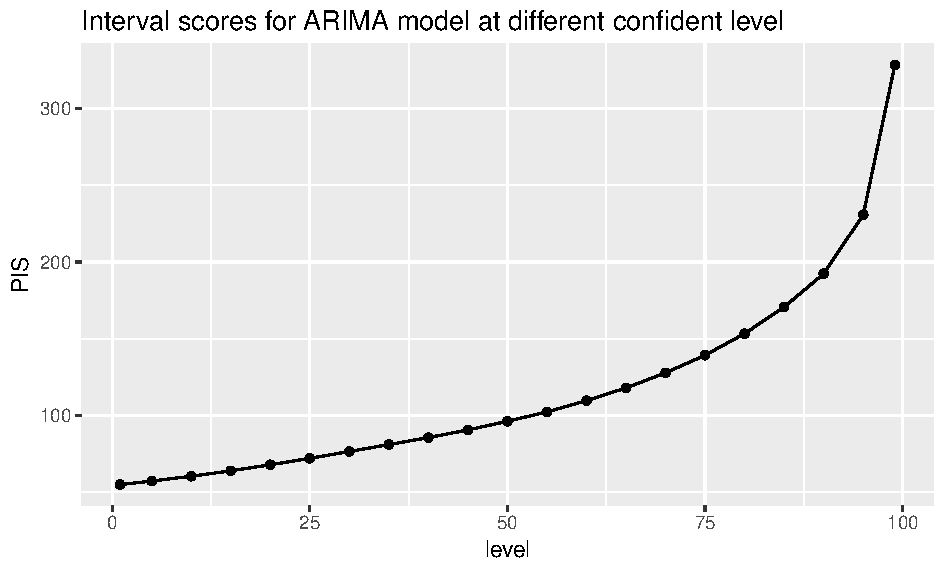
\includegraphics{thesis_files/figure-latex/plot1-1.pdf}

The upper curve was generated by processing the data. This graph shows
that as the confidence interval increases, the interval score shows a
trend of accelerating and increasing, and the score reaches the highest
at 99\%. The lower the score represents the better result of the
interval forecasts, so the information from this curve shows that, the
interval forecasts for the simple return of the ASX200 by using ARIMA
model is better when the confident interval level is smaller

Then use the same way to set confidence intervals, and use GARCH model
to forecast the intervals at different confidence level. After using
interval scoring rules to evaluate the results and making graph. After
that, a score change curve is obtained, which shows the result very
similar to that obtained by using the ARIMA model before.

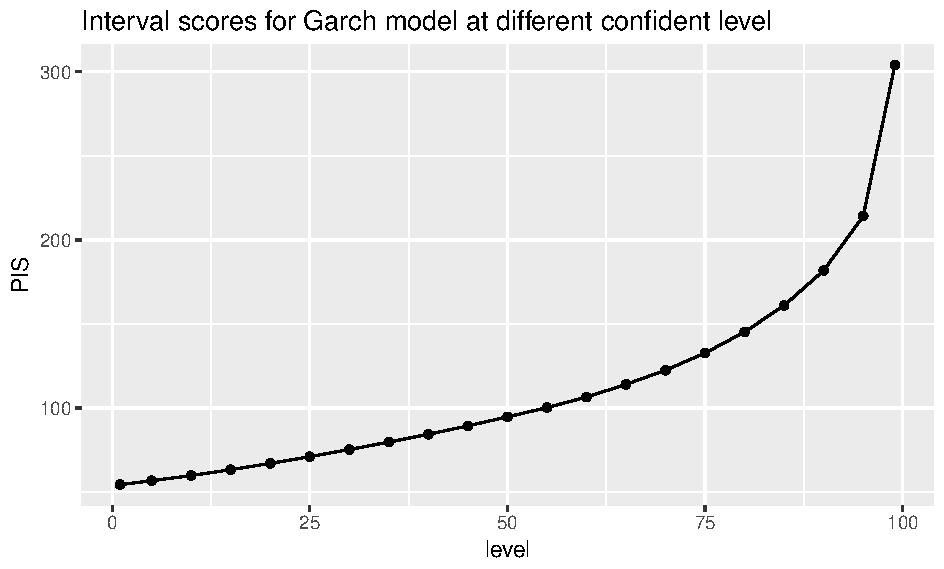
\includegraphics{thesis_files/figure-latex/plot2-1.pdf}

This graph also shows that as the confidence interval expands, the score
increases. It means that the smaller confidence intervals show better
score results by using GRACH model. Because the images produced by using
the two different models are extremely similar, we put them together for
comparison.

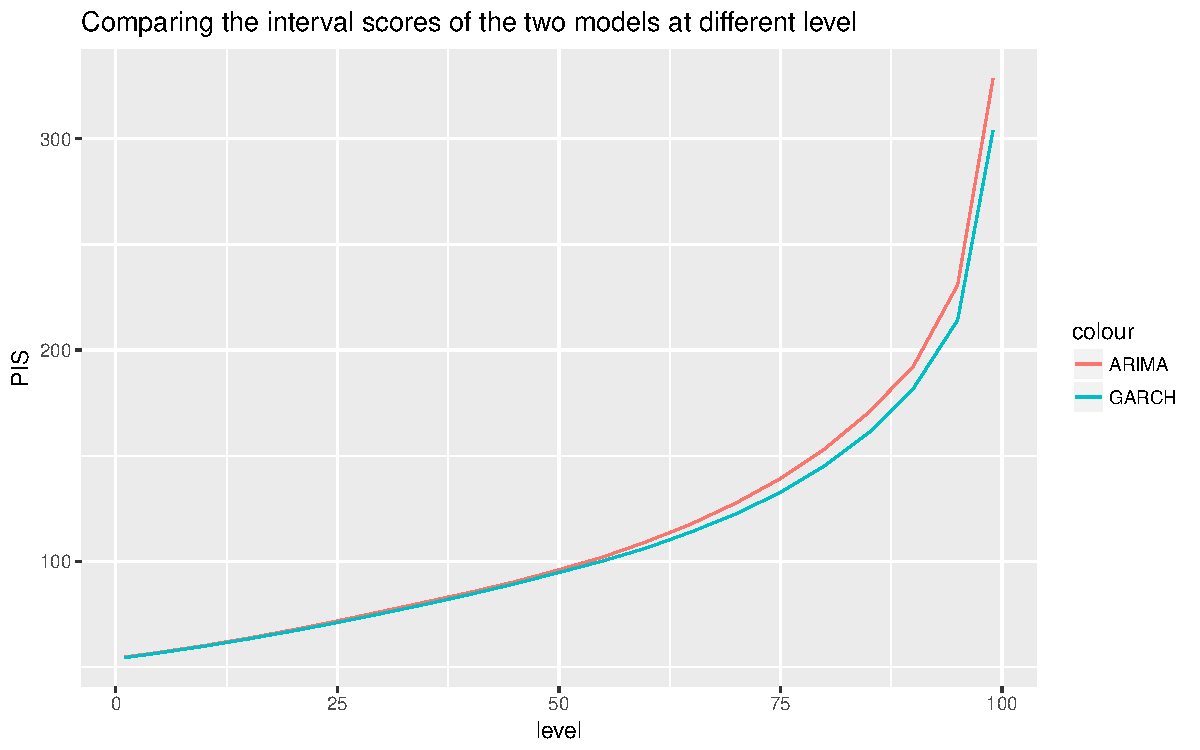
\includegraphics{thesis_files/figure-latex/plot3-1.pdf}

By comparing these two curves, their overall characteristics are
extremely similar. Their scores are not very different at smaller
confidence intervals, but in the larger confidence interval, the scores
are slightly different by using these two different models.

\section{Probabilistic forecasts for the ASX 200
index}\label{probabilistic-forecasts-for-the-asx-200-index}

For probabilistic forecasts, we still using the ARIMA(0,0,3) model and
MA(3)-GARCH(1,1) model to fit data and make forecast, which were
produced at Chapter 3.1. Afterwards, the train set is also predicted by
two different models. However, unlike the result obtained in 3.2, we do
not need to set the confidence interval. Instead, use packages R
packages ``scoringRules'' (\textcite{JKL17}), we can obtained the
evaluation results by using three distribution scoring rules
(Logarithmic score, Continuous Ranked Probability Score and
Dawid-Sebastianti score) directly.

\begin{table}

\caption{\label{tab:table2}Scoring Rules for MA model and GARCH model}
\centering
\begin{tabular}[t]{lrrr}
\toprule
  & CRPS & LogS & DSS\\
\midrule
GARCH & 20.70 & 5.10 & 8.36\\
ARIMA & 21.13 & 5.14 & 8.45\\
\bottomrule
\end{tabular}
\end{table}

According to the table above, the results of three type scoring rules of
MA(3)-garch(1,1) model are all smaller than the result of MA(3) Model.
Therefore, it can be shown here that the garch model has a better
prediction performance compared to MA(3).

\chapter{Case study two: M3 data
sets}\label{case-study-two-m3-data-sets}

The M3 dataset includes 3003 different type time series, it is from R
packages ``Mcomp'' (\textcite{RH182}), it can provide more information
for evaluating probabilistic forecast by using scoring rule. Different
from previous financial data, M3 datasets can use different models for
predictive analysis at the same time. In this part, three prediction
models are chosen, ARIMA model, ETS model, and Random walk model.

As in the previous chapter, before we start forecasting and evaluating,
the suitable models should be selected. However, for the M3 datasets,
there are more than 3000 different time series, so we have modeled all
the time series separately by these three models. Meanwhile, because
these different time series come from different fields, their the units
of test set are all different. Therefore, Before the final evaluation
process, the units of each different time series should be unified,
which can reduce unnecessary errors when comparing the results of the
final evaluation.

\section{Interval forcast for the M3 competition
data}\label{interval-forcast-for-the-m3-competition-data}

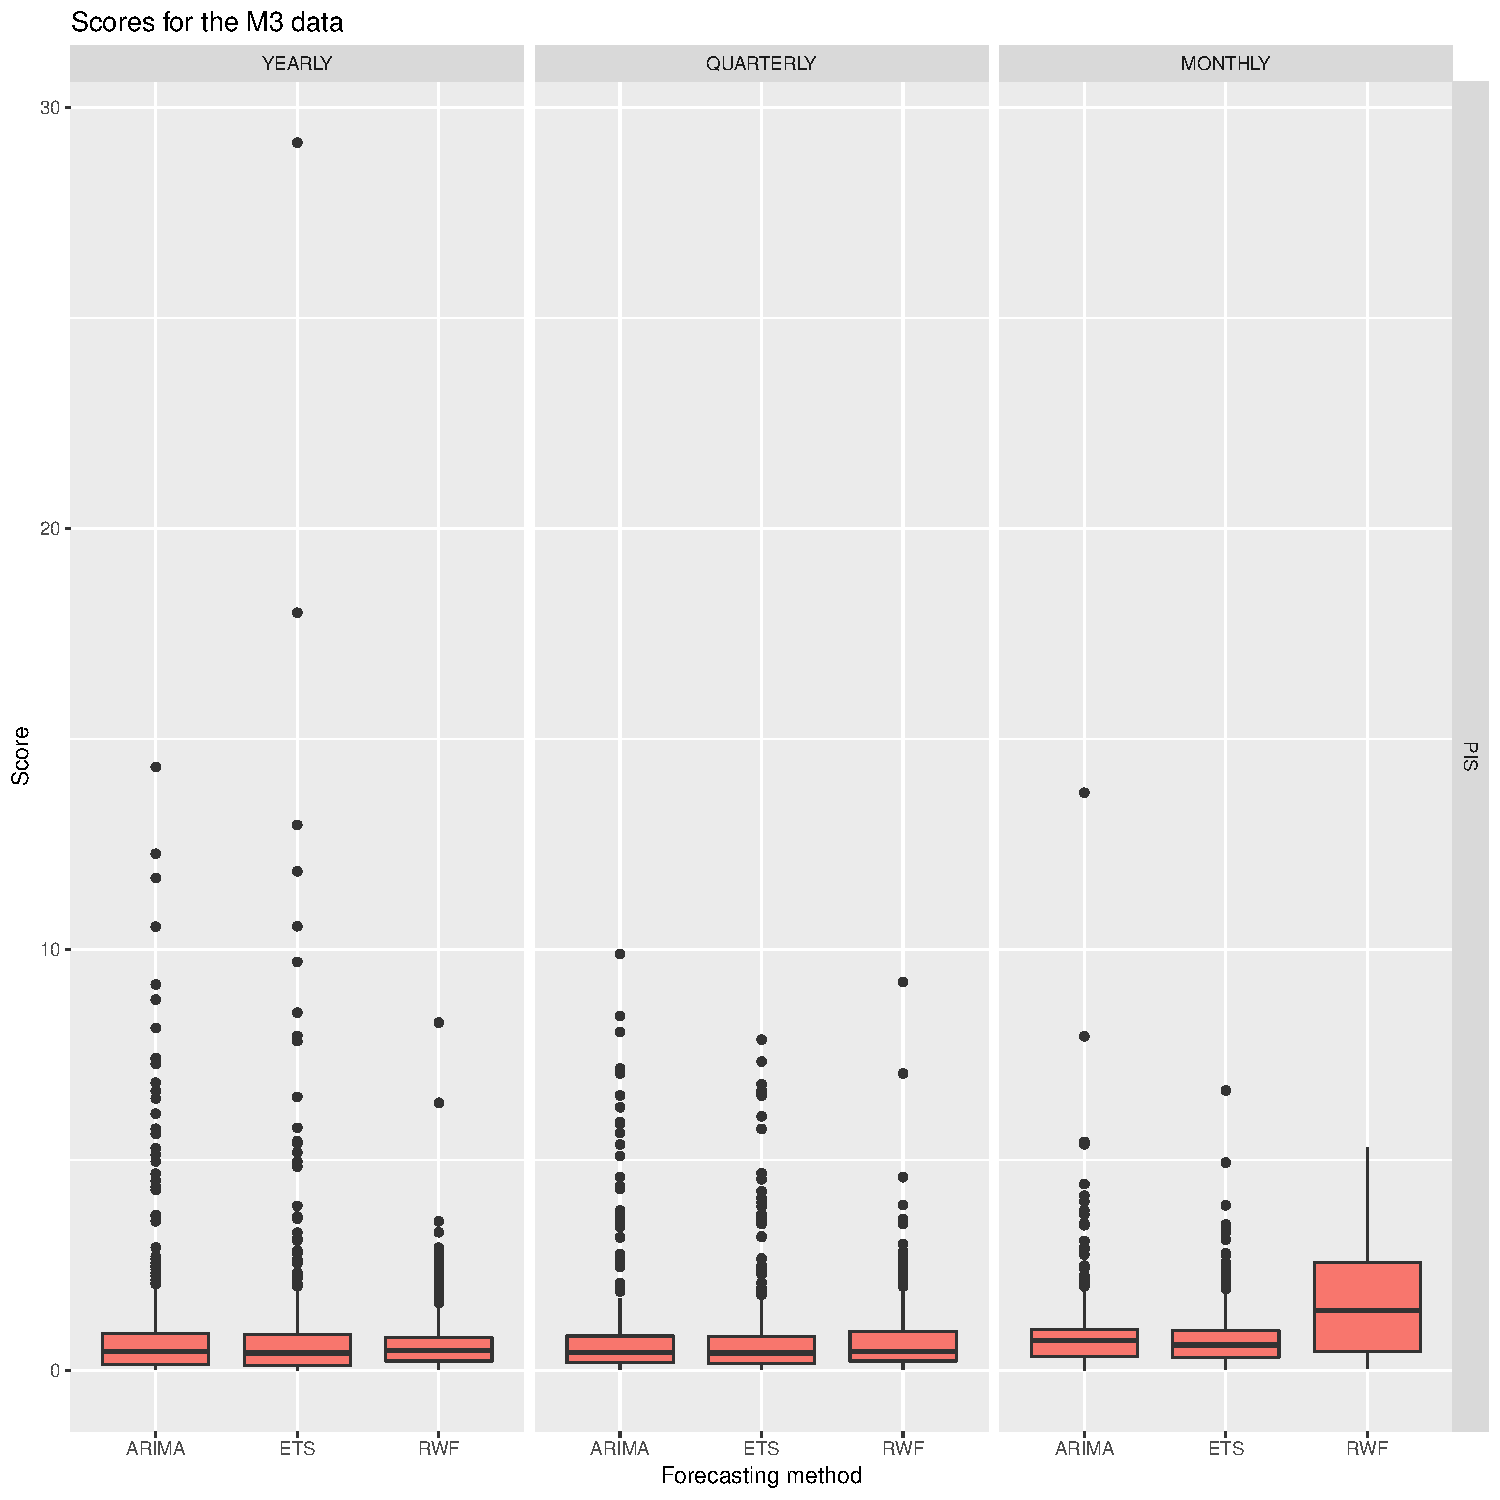
\includegraphics[width=1\linewidth]{thesis_files/figure-latex/boxplotPIS-1}

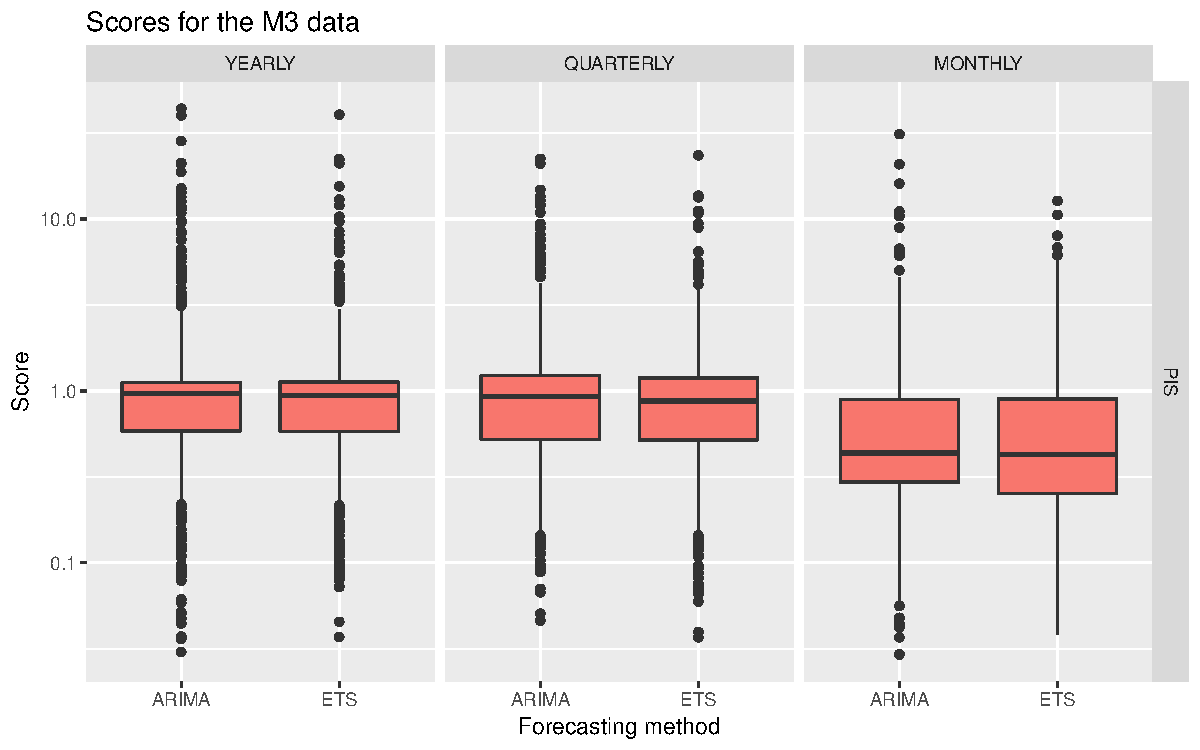
\includegraphics[width=1\linewidth]{thesis_files/figure-latex/boxplotlogPIS-1}

\section{Probabilistic forecasts for the M3 competition
data}\label{probabilistic-forecasts-for-the-m3-competition-data}

In this part, three prediction models (ARIMA model, ETS model, and
Random walk model) still be used as before. After separately predicting
these 3003 different time series, we reached 9009 forecast sets. Then
each of these forecasting sets is evaluated by three different scoring
rules separately. And to average the evaluation results for each
different time series. Use these evaluation results to generate three
boxplots, they represent the performance of different models to predict
under different scoring rules.

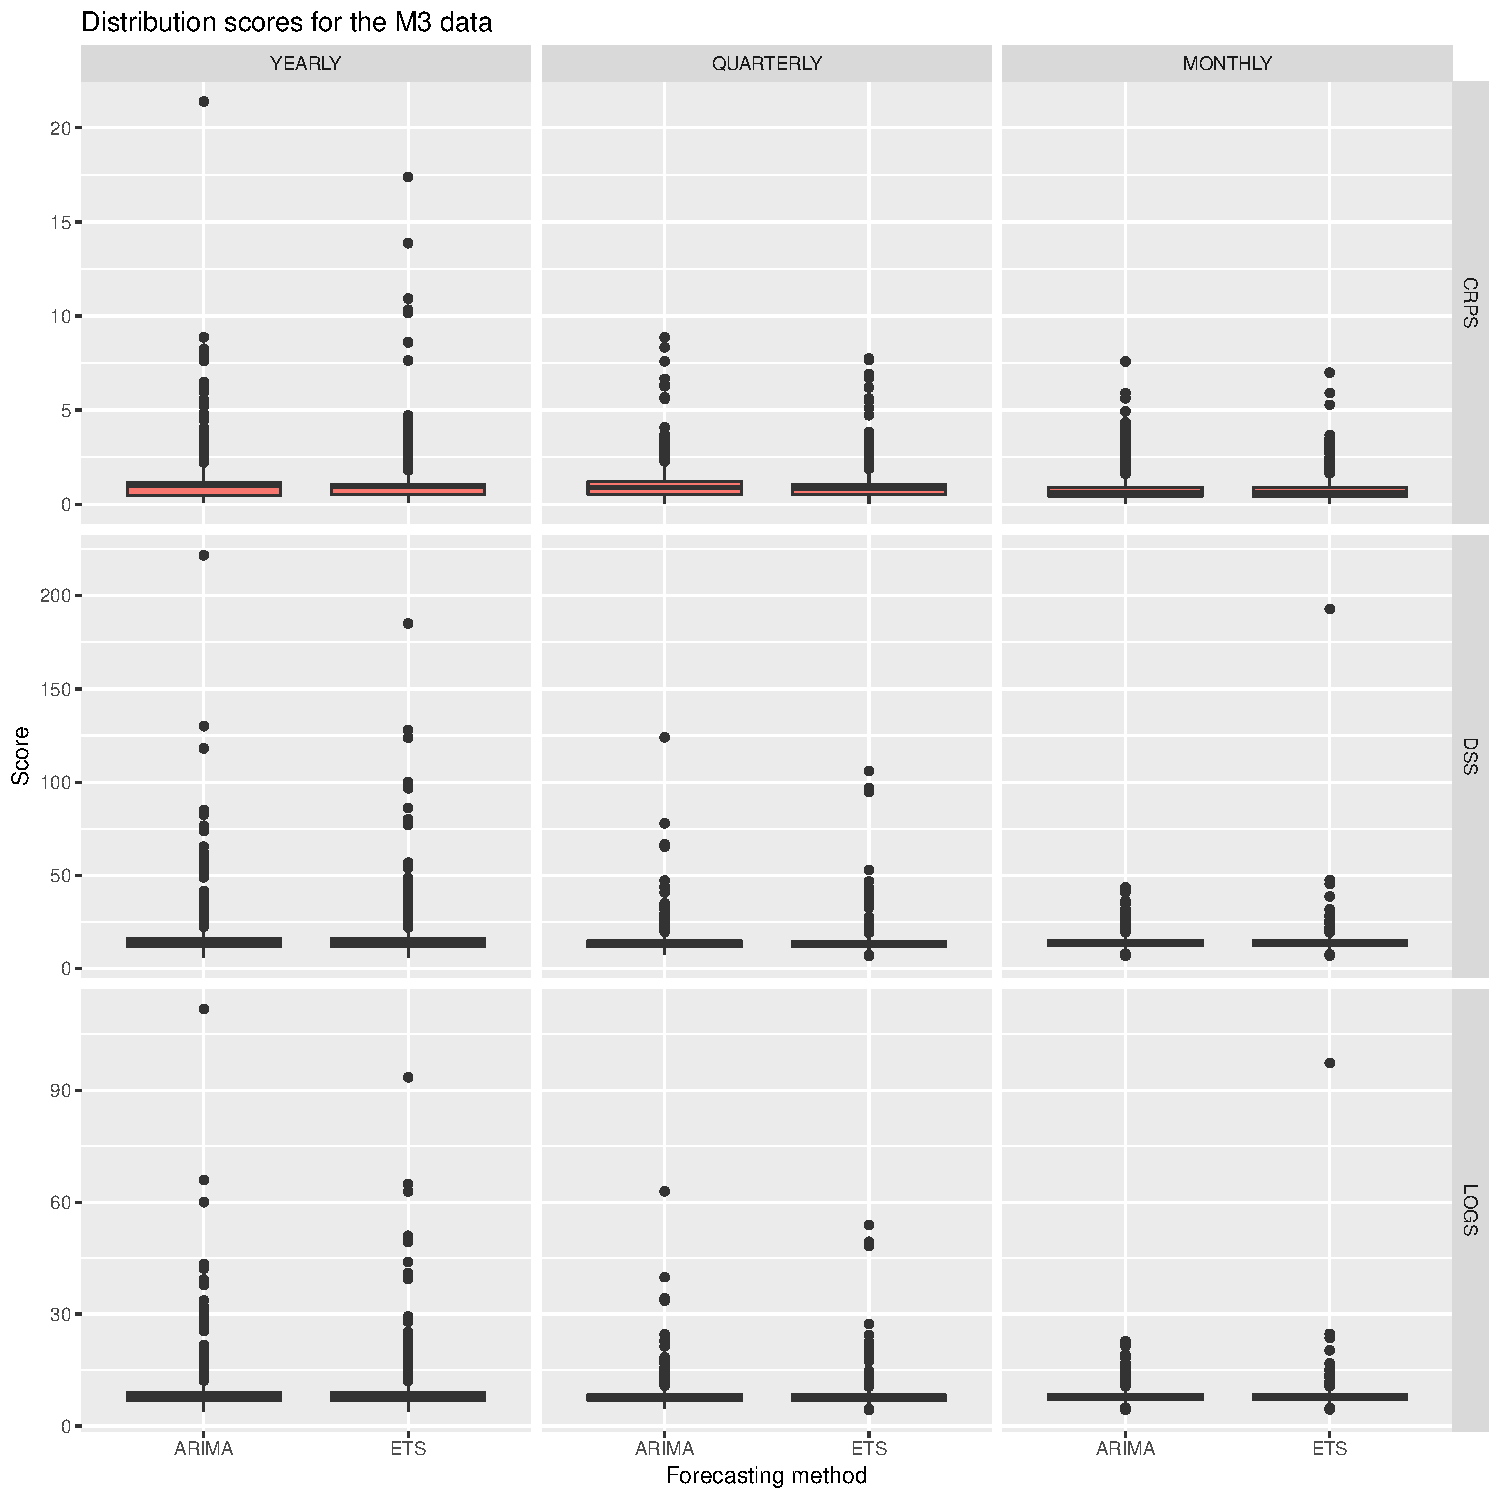
\includegraphics[width=1\linewidth]{thesis_files/figure-latex/boxplot-1}

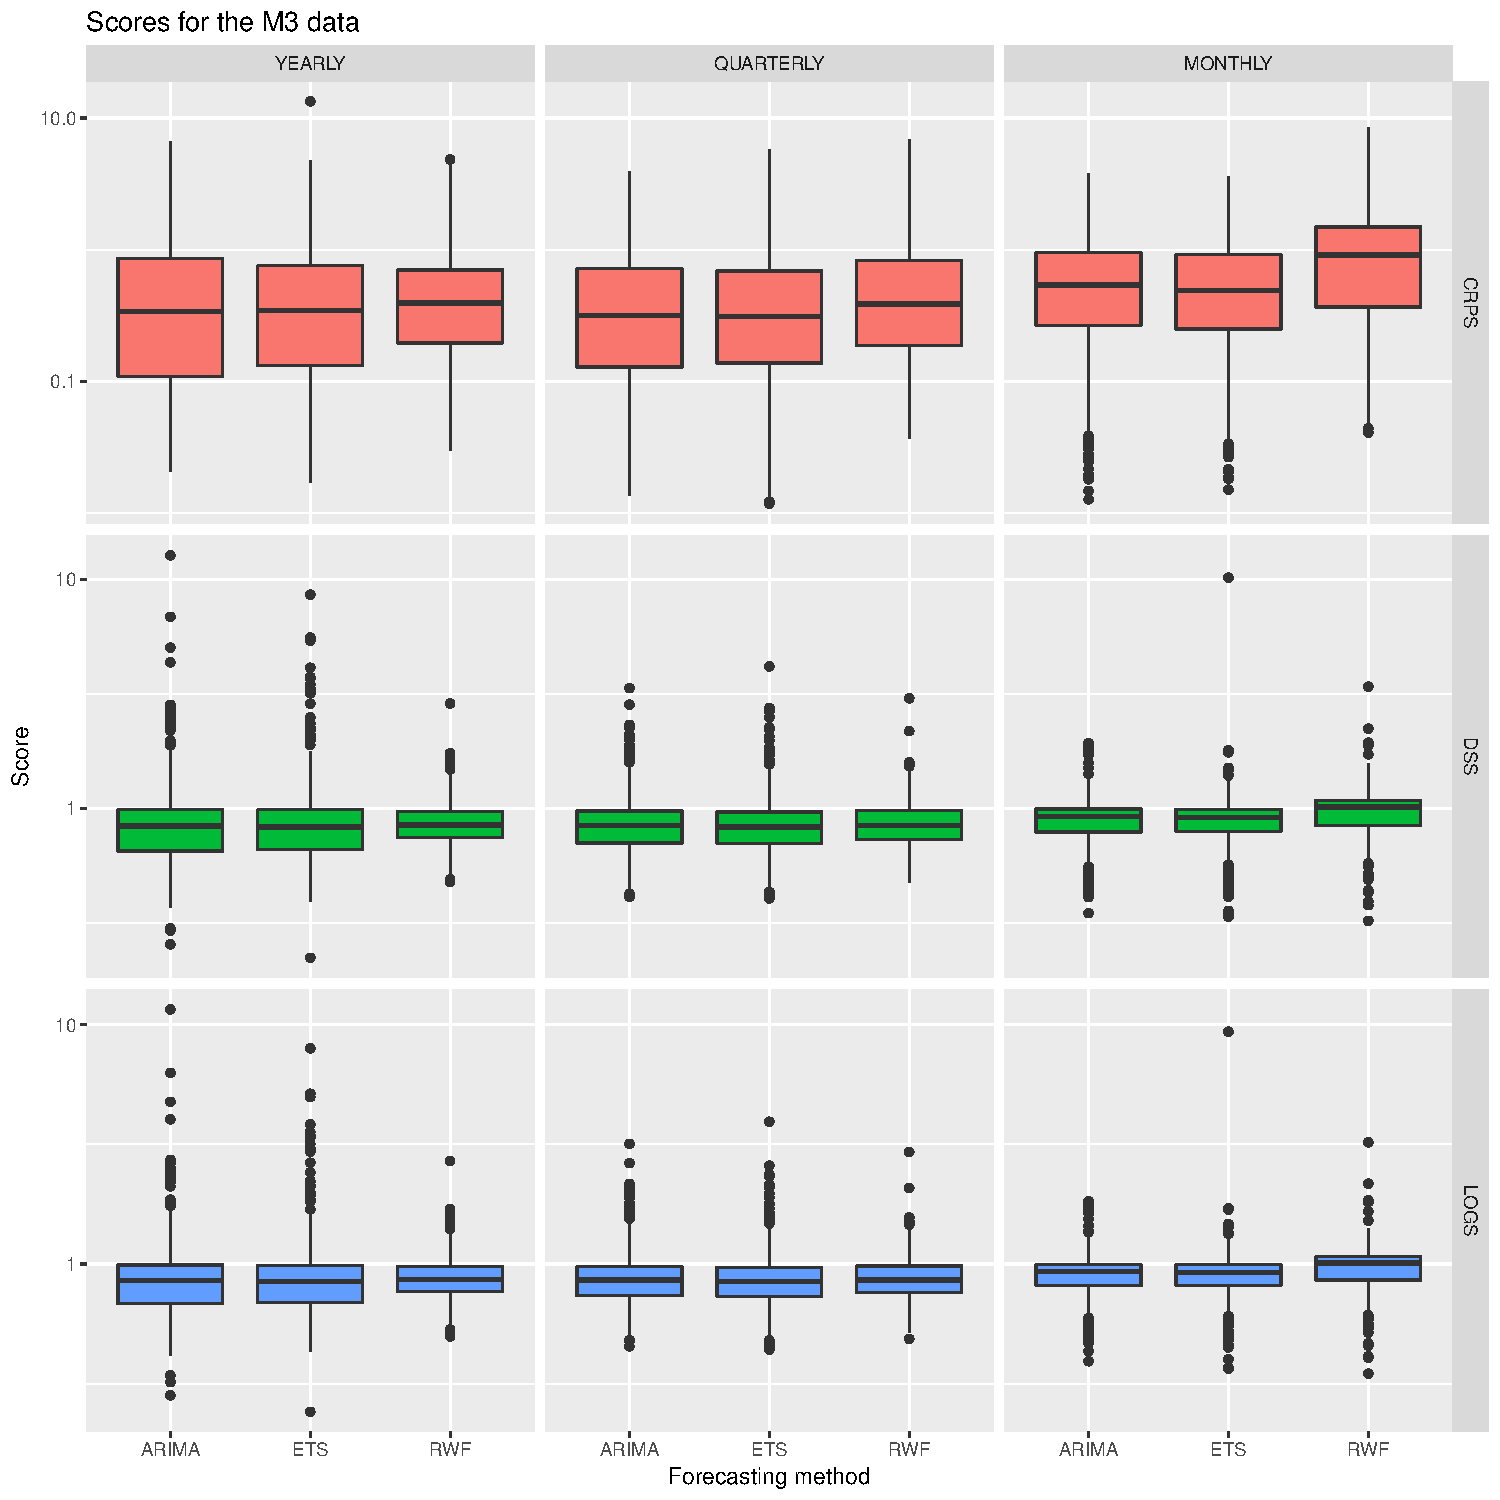
\includegraphics[width=1\linewidth]{thesis_files/figure-latex/boxplotlog-1}

Although it cannot be known from the above figure how many outliers are
generated base on the different forecast model by different scoring
rules, boxplots can show 5th, 25th, 50th, 75th and 95th percentiles of
central prediction interval width. The width of the obvious random walk
model is much narrower than that of other models, which means that its
sharpness is sharpest, and the calibration is more accurate, although
its mean value is not the lowest. Therefore, in the case of using M3
data sets, the quality of probability predictions derived from random
walk model is even higher. This also proves that using scoring rules can
simultaneously evaluate the sharpness and calibration of probabilistic
results.

\chapter{Conclusion}\label{conclusion}

In this report, we introduced what is the probabilistic forecasts, and
calibration and sharpness. It also introduced scoring rules. For the
three commonly used scoring rules, we show their original formulas and
form under Gaussian predictive distribution. In the section of the case
study, we first used two models to do probabilistic forecasts for the
ASX200 index, to evaluate the forecasts results by using scoring rules.
Then we learned how to use scoring rules to evaluate the outcome of
forecasts. In the second case study, we used the M3 datasets and used
multiple models to do probabilistic forecasts. We learned how the
scoring rules evaluated both the probabilities and the results of car
calibration and sharpness.

\printbibliography[heading=bibintoc]



\end{document}
